\documentclass[a4paper]{article}
\usepackage[affil-it]{authblk}
\usepackage[backend=bibtex,style=numeric]{biblatex}
\usepackage{amsmath,amssymb,amsfonts}
\usepackage{tikz}
\usepackage{pgfplots}
\usepackage{amsmath}
\usepackage{geometry}
\geometry{margin=1.5cm, vmargin={0pt,1cm}}
\setlength{\topmargin}{-1cm}
\setlength{\paperheight}{29.7cm}
\setlength{\textheight}{25.3cm}

\addbibresource{citation.bib}

\begin{document}
% =================================================
\title{Numerical Analysis homework V}

\author{LI YIJIAN 3230102477
  \thanks{Electronic address: \texttt{3230102477@zju.edu.cn}}}
\affil{(Mathematics and Applied Mathematics 2302), Zhejiang University }


\date{Due time: \today}
\maketitle





% ============================================
\section*{I. Detailed proof of Thm}
We first check that the operations that
\(\mathcal{C}[a,b]\) is closed under them.

\medskip\noindent
\textbf{Closure under addition.}
Let \(f,g\in \mathcal{C} [a,b]\).  
For each \(x\in[a,b]\) we define
\((f+g)(x):=f(x)+g(x)\).
Since \(f\) and \(g\) are continuous and the sum of continuous
functions is continuous, the function \(f+g\) is continuous on \([a,b]\).
Hence \(f+g\in C[a,b]\).

\medskip\noindent
\textbf{Closure under scalar multiplication.}
Let \(f\in \mathcal{C}[a,b]\) and \(\alpha\in\mathbb{C}\).
For each \(x\in[a,b]\) define
\((\alpha f)(x):=\alpha f(x)\).
The map \(x\mapsto f(x)\) is continuous, and multiplication by the
constant \(\alpha\) is a continuous operation, so the product
\(\alpha f\) is continuous on \([a,b]\).
Thus \(\alpha f\in \mathcal{C}[a,b]\).

\medskip
Now we verify the vector space axioms.
All equalities below are understood pointwise on \([a,b]\).

\begin{itemize}
  \item \emph{Associativity of addition:}
        For any \(f,g,h\in \mathcal{C}[a,b]\),
        \[
        ((f+g)+h)(x)
        = (f(x)+g(x))+h(x)
        = f(x)+(g(x)+h(x))
        = (f+(g+h))(x).
        \]
  \item \emph{Commutativity of addition:}
        For any \(f,g\in \mathcal{C}[a,b]\),
        \[
        (f+g)(x)=f(x)+g(x)=g(x)+f(x)=(g+f)(x).
        \]
  \item \emph{Additive identity:}
        Let \(0\) denote the zero function
        \(0(x)\equiv 0\).
        It is continuous and
        \((f+0)(x)=f(x)+0=f(x)\) for all \(x\), so \(f+0=f\).
  \item \emph{Additive inverse:}
        For \(f\in \mathcal{C}[a,b]\), define \(-f\) by
        \((-f)(x):=-f(x)\). Then \(-f\) is continuous and
        \((f+(-f))(x)=f(x)-f(x)=0\), so \(f+(-f)=0\).
  \item \emph{Compatibility of scalar multiplication:}
        For \(\alpha,\beta\in\mathbb{C}\) and \(f\in C[a,b]\),
        \[
        ((\alpha\beta)f)(x)
        =(\alpha\beta)f(x)
        =\alpha(\beta f(x))
        =(\alpha(\beta f))(x).
        \]
  \item \emph{Identity scalar:}
        For \(f\in \mathcal{C}[a,b]\),
        \[
        (1\cdot f)(x)=1\cdot f(x)=f(x),
        \]
        hence \(1\cdot f=f\).
  \item \emph{Distributivity over function addition:}
        For \(\alpha\in\mathbb{C}\) and \(f,g\in \mathcal{C}[a,b]\),
        \[
        (\alpha(f+g))(x)
          =\alpha(f(x)+g(x))
          =\alpha f(x)+\alpha g(x)
          =(\alpha f+\alpha g)(x).
        \]
  \item \emph{Distributivity over scalar addition:}
        For \(\alpha,\beta\in\mathbb{C}\) and \(f\in \mathcal{C}[a,b]\),
        \[
        ((\alpha+\beta)f)(x)
          =(\alpha+\beta)f(x)
          =\alpha f(x)+\beta f(x)
          =(\alpha f+\beta f)(x).
        \]
\end{itemize}

All vector space axioms over \(\mathbb{C}\) are therefore satisfied,
so \(\mathcal{C}   [a,b]\) is a complex vector space.
We first check that \(\langle\cdot,\cdot\rangle\) satisfies the axioms of
an inner product on a complex vector space.

\medskip\noindent
\textbf{(1) Conjugate symmetry.}
For any \(u,v \in \mathcal{C}[a,b]\) we have
\[
\overline{\langle v,u\rangle}
  = \overline{\int_a^b \rho(t)\,v(t)\,\overline{u(t)}\,\mathrm{d}t}
  = \int_a^b \rho(t)\,\overline{v(t)}\,u(t)\,\mathrm{d}t
  = \int_a^b \rho(t)\,u(t)\,\overline{v(t)}\,\mathrm{d}t
  = \langle u,v\rangle .
\]

\medskip\noindent
\textbf{(2) Linearity in the first slot.}
Let \(u_1,u_2,v \in \mathcal{C}[a,b]\) and \(\alpha,\beta\in\mathbb C\).
Using linearity of the (Lebesgue or Riemann) integral, we obtain
\[
\begin{aligned}
\langle \alpha u_1+\beta u_2, v\rangle
 &= \int_a^b \rho(t)\bigl(\alpha u_1(t)+\beta u_2(t)\bigr)\overline{v(t)}\,\mathrm{d}t \\
 &= \alpha \int_a^b \rho(t)u_1(t)\overline{v(t)}\,\mathrm{d}t
   + \beta  \int_a^b \rho(t)u_2(t)\overline{v(t)}\,\mathrm{d}t \\
 &= \alpha\langle u_1,v\rangle + \beta\langle u_2,v\rangle .
\end{aligned}
\]

\medskip\noindent
\textbf{(3) Conjugate linearity in the second slot.}
This follows from (1) and (2). Indeed, for
\(u,v_1,v_2\in C[a,b]\) and \(\alpha,\beta\in\mathbb C\),
\[
\begin{aligned}
\langle u,\alpha v_1+\beta v_2\rangle
 &= \overline{\langle \alpha v_1+\beta v_2,u\rangle} \\
 &= \overline{\alpha\langle v_1,u\rangle + \beta\langle v_2,u\rangle} \\
 &= \overline{\alpha}\,\langle u,v_1\rangle
  + \overline{\beta}\,\langle u,v_2\rangle .
\end{aligned}
\]

\medskip\noindent
\textbf{(4) Positive definiteness.}
For any \(u\in C[a,b]\),
\[
\langle u,u\rangle
 = \int_a^b \rho(t)\,|u(t)|^2\,\mathrm{d}t .
\]
Since \(\rho(t)>0\) and \(|u(t)|^2\ge 0\) for all \(t\), the integrand is
non–negative, hence \(\langle u,u\rangle \ge 0\).

If \(\langle u,u\rangle = 0\), then
\(\int_a^b \rho(t)\,|u(t)|^2\,\mathrm{d}t = 0\).
Because the integrand is continuous and non–negative and \(\rho(t)>0\),
this can happen only if
\(\rho(t)\,|u(t)|^2=0\) for all \(t\in[a,b]\).
Thus \(|u(t)|^2=0\) for all \(t\), so \(u(t)=0\) for all \(t\in[a,b]\),
that is, \(u\equiv 0\).
Conversely, if \(u\equiv 0\), then clearly \(\langle u,u\rangle=0\).
Hence \(\langle u,u\rangle=0\) if and only if \(u=0\).

Combining (1)–(4), we see that \(\langle\cdot,\cdot\rangle\) is indeed an
inner product on \(C[a,b]\).

\medskip
Now define
\[
\|u\|_2 := \sqrt{\langle u,u\rangle}
          = \Bigl( \int_a^b \rho(t)\,|u(t)|^2\,\mathrm{d}t \Bigr)^{1/2}.
\]
On any inner–product space the function
\(\|u\|:=\sqrt{\langle u,u\rangle}\) satisfies the three norm axioms:
\(\|u\|\ge 0\) and \(\|u\|=0\) iff \(u=0\),
\(\|\alpha u\| = |\alpha|\|u\|\), and the triangle inequality
\(\|u+v\|\le\|u\|+\|v\|\), the last one following from the
Cauchy–Schwarz inequality.
Therefore \(\|\cdot\|_2\) is a norm on \(\mathcal{C}[a,b]\).

Hence \(\mathcal{C}[a,b]\) equipped with \(\langle\cdot,\cdot\rangle\) is an
inner–product space over \(\mathbb C\), and the corresponding norm
\(\|\cdot\|_2\) makes \(\mathcal{C}[a,b]\) into a normed vector space.






\section*{II. Chebyshev polynomials of the first kind}
\subsection*{(a)}
It suffices to show that for $m\neq n$ with $m,n\in\mathbb{N}$,
\[
\int_{-1}^{1}\frac{T_m(x)T_n(x)}{\sqrt{1-x^2}}\,dx=0.
\]
Using $T_k(x)=\cos(k\arccos x)$, we have
\[
\int_{-1}^{1}\frac{T_m(x)T_n(x)}{\sqrt{1-x^2}}\,dx
=\int_{-1}^{1}\frac{\cos(m\arccos x)\cos(n\arccos x)}{\sqrt{1-x^2}}\,dx.
\]
Let $t=\arccos x$, so that $x=\cos t$ and $dx=-\sin t\,dt$. Since
$\sqrt{1-x^2}=\sqrt{1-\cos^2 t}=\sin t$ for $t\in[0,\pi]$, we obtain
\[
\int_{-1}^{1}\frac{\cos(m\arccos x)\cos(n\arccos x)}{\sqrt{1-x^2}}\,dx
=\int_{\pi}^{0}\frac{\cos(mt)\cos(nt)}{\sin t}(-\sin t)\,dt
=\int_{0}^{\pi}\cos(mt)\cos(nt)\,dt.
\]
Now use the identity $\cos a\cos b=\frac12\bigl(\cos(a+b)+\cos(a-b)\bigr)$:
\[
\int_{0}^{\pi}\cos(mt)\cos(nt)\,dt
=\frac12\int_{0}^{\pi}\bigl(\cos((m+n)t)+\cos((m-n)t)\bigr)\,dt.
\]
If $m\neq n$, then $m+n\neq 0$ and $m-n\neq 0$, hence
\[
\int_{0}^{\pi}\cos(kt)\,dt=\left[\frac{\sin(kt)}{k}\right]_{0}^{\pi}=0
\quad (k\in\mathbb{Z}\setminus\{0\}),
\]
so the integral is $0$, as desired.
\subsection*{(b)}
The first three Chebyshev polynomials of the first are
\[
T_0(x)=1,\qquad T_1(x)=x,\qquad T_2(x)=2x^2-1.
\]
Using the result in (a)
\[
\langle T_0,T_0\rangle=\pi,\qquad \langle T_n,T_n\rangle=\frac{\pi}{2}\ \ (n\ge 1),
\]
we get
\[
\|T_0\|=\sqrt{\pi},\qquad \|T_1\|=\sqrt{\frac{\pi}{2}},\qquad \|T_2\|=\sqrt{\frac{\pi}{2}}.
\]
Hence an orthonormal system is
\[
\phi_0(x)=\frac{T_0(x)}{\|T_0\|}=\frac{1}{\sqrt{\pi}},\qquad
\phi_1(x)=\frac{T_1(x)}{\|T_1\|}=\sqrt{\frac{2}{\pi}}\,x,\qquad
\phi_2(x)=\frac{T_2(x)}{\|T_2\|}=\sqrt{\frac{2}{\pi}}\,(2x^2-1).
\]
Then $\langle \phi_i,\phi_j\rangle=\delta_{ij}$ for $i,j\in\{0,1,2\}$ Then is an orthonormal system.

\subsection*{III. Least-squares approximation of $y(x)=\sqrt{1-x^2}$ on $[-1,1]$}

We use the inner product from Theorem 5.7 with
\[
\langle f,g\rangle=\int_{-1}^{1} f(x)g(x)\rho(x)dx,
\qquad 
\rho(x)=\frac{1}{\sqrt{1-x^2}}.
\]
Let $f(x)=\sqrt{1-x^2}$. So \(\langle f,g\rangle=\int_{-1}^{1} g(x)dx\)

\subsection*{(a) Fourier expansion}

By result in II(b) $T_n(\cos t)=\cos(nt)$. \[
\phi_0(x)=\frac{T_0(x)}{\|T_0\|}=\frac{1}{\sqrt{\pi}},\qquad
\phi_1(x)=\frac{T_1(x)}{\|T_1\|}=\sqrt{\frac{2}{\pi}}\,x,\qquad
\phi_2(x)=\frac{T_2(x)}{\|T_2\|}=\sqrt{\frac{2}{\pi}}\,(2x^2-1).
\]
Compute the coefficients:
\[
a_0=\langle f,\phi_0\rangle
=\int_{-1}^{1}\phi_0(x)\,dx
=\int_{-1}^{1}\frac{1}{\sqrt{\pi}}\,dx
=\frac{2}{\sqrt{\pi}},
\]
\[
a_1=\langle f,\phi_1\rangle
=\int_{-1}^{1}\phi_1(x)\,dx
=\int_{-1}^{1}\sqrt{\frac{2}{\pi}}\,x\,dx
=0,
\]
\[
a_2=\langle f,\phi_2\rangle
=\int_{-1}^{1}\phi_2(x)\,dx
=\int_{-1}^{1}\sqrt{\frac{2}{\pi}}(2x^2-1)\,dx
=\sqrt{\frac{2}{\pi}}\left(2\cdot\frac{2}{3}-2\right)
=-\frac{2}{3}\sqrt{\frac{2}{\pi}}.
\]
Thus
\[
p_2(x)=\frac{2}{\sqrt{\pi}}\cdot\frac{1}{\sqrt{\pi}}
+\left(-\frac{2}{3}\sqrt{\frac{2}{\pi}}\right)\cdot\sqrt{\frac{2}{\pi}}\,(2x^2-1)
=\frac{2}{\pi}-\frac{4}{3\pi}(2x^2-1)
=\frac{10}{3\pi}-\frac{8}{3\pi}x^2.
\]

\subsection*{(b) normal equations}

Let $p_2(x)=c_0+c_1x+c_2x^2$. Then we know
\[
\langle f-p_2,\,1\rangle=0,\qquad
\langle f-p_2,\,x\rangle=0,\qquad
\langle f-p_2,\,x^2\rangle=0,
\]

Since $f(x)$ and $\rho(x)=\dfrac{1}{\sqrt{1-x^2}}$ are even, while $x$ is odd,
we have $\langle f,x\rangle=0$, $\langle 1,x\rangle=0$, and $\langle x^2,x\rangle=0$.
Thus $\langle f-p_2,x\rangle=0$ forces $c_1=0$.

Now compute the needed inner products directly:
\[
\langle f,1\rangle=
=\int_{-1}^{1}1\,dx=2,
\]
\[
\langle 1,1\rangle=\int_{-1}^{1}\frac{1}{\sqrt{1-x^2}}\,dx=\pi,
\qquad
\langle x^2,1\rangle=\int_{-1}^{1}\frac{x^2}{\sqrt{1-x^2}}\,dx=\frac{\pi}{2}.
\]
Hence $\langle f-p_2,1\rangle=0$ becomes
\[
2-c_0\pi-c_2\frac{\pi}{2}=0.
\]
Then
\[
\langle f,x^2\rangle
=\int_{-1}^{1}x^2\,dx=\frac{2}{3},
\]
\[
\langle 1,x^2\rangle=\int_{-1}^{1}\frac{x^2}{\sqrt{1-x^2}}\,dx=\frac{\pi}{2},
\qquad
\langle x^2,x^2\rangle=\int_{-1}^{1}\frac{x^4}{\sqrt{1-x^2}}\,dx=\frac{3\pi}{8}.
\]
Therefore $\langle f-p_2,x^2\rangle=0$ becomes
\[
\frac{2}{3}-c_0\frac{\pi}{2}-c_2\frac{3\pi}{8}=0.
\]
Solving the eqaution
\[
c_2=-\frac{8}{3\pi},\qquad c_0=\frac{10}{3\pi},\qquad c_1=0,
\]
hence
\[
p_2(x)=\frac{10}{3\pi}-\frac{8}{3\pi}x^2,
\]










\section*{IV. DLS}
\paragraph{data.}
We have $N=12$, $\rho\equiv 1$, and the sales record (Example 5.55) is
\[
(x_i,y_i)=
(1,256),(2,201),(3,159),(4,61),(5,77),(6,40),(7,17),(8,25),(9,103),(10,156),(11,222),(12,345).
\]
Define the discrete inner product
\[
\langle u,v\rangle=\sum_{i=1}^{12} u(x_i)v(x_i).
\]

\subsection*{IV(a) Orthonormal polynomials via Gram--Schmidt}
Start from the independent list $(1,x,x^2)$.

\medskip
\noindent\textbf{Step 1.}
Let $p_0(x)=1$. Then
\[
\langle p_0,p_0\rangle=\sum_{i=1}^{12}1=12,
\qquad
\phi_0(x)=\frac{p_0(x)}{\|p_0\|}=\frac{1}{\sqrt{12}}.
\]

\medskip
\noindent\textbf{Step 2.}
Let $v_1(x)=x$. Remove its projection onto $\phi_0$:
\[
\langle v_1,\phi_0\rangle=\sum_{i=1}^{12} x_i\cdot \frac{1}{\sqrt{12}}
=\frac{1}{\sqrt{12}}\sum_{i=1}^{12} i
=\frac{78}{\sqrt{12}}.
\]
Hence
\[
p_1(x)=v_1(x)-\langle v_1,\phi_0\rangle \phi_0(x)
=x-\frac{78}{12}=x-\frac{13}{2}.
\]
Moreover,
\[
\langle p_1,p_1\rangle=\sum_{i=1}^{12}\Bigl(i-\frac{13}{2}\Bigr)^2=143,
\qquad
\phi_1(x)=\frac{p_1(x)}{\|p_1\|}=\frac{x-\frac{13}{2}}{\sqrt{143}}.
\]

\medskip
\noindent\textbf{Step 3.}
Let $v_2(x)=x^2$. Remove its projections onto $\phi_0,\phi_1$ and set
\[
p_2(x)=v_2(x)-\langle v_2,\phi_0\rangle\phi_0(x)-\langle v_2,\phi_1\rangle\phi_1(x).
\]
A direct computation gives
\[
p_2(x)=x^2-13x+\frac{91}{3}.
\]
Furthermore,
\[
\langle p_2,p_2\rangle=\sum_{i=1}^{12}\Bigl(i^2-13i+\frac{91}{3}\Bigr)^2=\frac{4004}{3}.
\]
Equivalently, multiplying by $3$ to avoid fractions,
\[
\phi_2(x)=\frac{3p_2(x)}{\|3p_2\|}
=\frac{3x^2-39x+91}{\sqrt{12012}},
\]
since $\langle 3p_2,3p_2\rangle=9\cdot\frac{4004}{3}=12012$.

\medskip
\noindent Therefore an orthonormal system is
\[
\boxed{
\phi_0(x)=\frac1{\sqrt{12}},\qquad
\phi_1(x)=\frac{x-\frac{13}{2}}{\sqrt{143}},\qquad
\phi_2(x)=\frac{3x^2-39x+91}{\sqrt{12012}}.
}
\]

\subsection*{IV(b) Best quadratic least--squares approximation}
We seek $\hat\varphi(x)=a_0+a_1x+a_2x^2$ minimizing
\[
\sum_{i=1}^{12}\bigl(y_i-\hat\varphi(x_i)\bigr)^2
=\|y-\hat\varphi\|^2
\]
with respect to the discrete inner product.

\medskip
\noindent\textbf{Using the orthonormal basis.}
Write
\[
\hat\varphi(x)=c_0\phi_0(x)+c_1\phi_1(x)+c_2\phi_2(x),
\qquad
c_k=\langle y,\phi_k\rangle.
\]
Compute
\[
c_0=\sum_{i=1}^{12} y_i\cdot \frac1{\sqrt{12}}
=\frac{\sum_{i=1}^{12}y_i}{\sqrt{12}}
=\frac{1662}{\sqrt{12}},
\]
\[
c_1=\sum_{i=1}^{12} y_i\cdot \frac{x_i-\frac{13}{2}}{\sqrt{143}}
=\frac{\sum_{i=1}^{12} y_i\left(x_i-\frac{13}{2}\right)}{\sqrt{143}}
=\frac{589}{\sqrt{143}},
\]
\[
c_2=\sum_{i=1}^{12} y_i\cdot \frac{3x_i^2-39x_i+91}{\sqrt{12012}}
=\frac{\sum_{i=1}^{12} y_i\,(3x_i^2-39x_i+91)}{\sqrt{12012}}
=\frac{36204}{\sqrt{12012}}.
\]
Converting back to the monomial basis yields
\[
\boxed{
\hat\varphi(x)=386-\frac{16220}{143}\,x+\frac{1293}{143}\,x^2
}
\]
(i.e. $\hat\varphi(x)\approx 386-113.4265734\,x+9.041958042\,x^2$).

\medskip
\noindent\textbf{(Verification via normal equations.)}
Let $A=[\mathbf{1},x,x^2]\in\mathbb{R}^{12\times 3}$ with rows $(1,x_i,x_i^2)$.
Then the normal equations are
\[
(A^\top A)a=A^\top y,
\qquad a=(a_0,a_1,a_2)^\top.
\]
Here
\[
A^\top A=
\begin{pmatrix}
12&78&650\\
78&650&6084\\
650&6084&60710
\end{pmatrix},
\qquad
A^\top y=
\begin{pmatrix}
1662\\
11392\\
109750
\end{pmatrix},
\]
whose solution is exactly
\[
a_0=386,\qquad a_1=-\frac{16220}{143},\qquad a_2=\frac{1293}{143},
\]
agreeing with the result above.

\subsection*{IV(c) Reuse when $y_i$ changes but $x_i$ and $N$ stay the same}
If another sales record has the same nodes $x_i$ and $N$ (and the same weight $\rho\equiv 1$)
but different values $y_i$, then:

\begin{itemize}
\item The orthonormal polynomials $\phi_0,\phi_1,\phi_2$ from part (a) can be reused,
since they depend only on $\{x_i\}$ and $\rho$.
\item Only the coefficients $c_k=\langle y,\phi_k\rangle=\sum_{i=1}^{12}y_i\phi_k(x_i)$
need to be recomputed.
\end{itemize}

This reuse illustrates an advantage of orthonormal polynomials over normal equations:
the (expensive) orthogonalization can be done once, and subsequent fits for new $y$
reduce to computing a few inner products, with better numerical stability than solving
normal equations repeatedly.


\section*{V. New method of rounding off number}
By the defination in the course, the unit roundoff represents the maximul round off error
around 1, where the floating number is the densest. By the new method of rounding off number
: the badest case is the number around 1 is $1 + 2^{-23}$ in IEEE-754. So
\[
\epsilon^{new}_{u} = 2^{-23} = 2\epsilon_{u}
\]


\section*{VI. Estimate the precision lost in the subtraction}
We know:
\[
\cos x = 1 - \frac{x^2}{2!} + \frac{x^4}{4!} + O(x^6)
\]
$\Rightarrow$
\[
1-\cos \frac{1}{4} = 2^{-5} + \epsilon \quad (\epsilon \ll 2^{-5})
\]
So the subtraction will lose 5 bits of precision.

\section*{VII. Symmetric Polynomials}
Method 1:
\[
1- \cos x = 2\sin^2(\frac{x}{2})
\]
Then we know near 0 $2\sin^2(\frac{x}{2})$ is small. So without the 
subtraction of two closed number. It will NOT cause a catastrophic cancellation.
\\
Method 2:
\[
1- \cos x = \frac{1-\cos^2x}{1+ \cos x} = \frac{\sin^2 x}{1+ \cos x}
\]
For the denominator, both of them are the number closed to 1, which will NOT cause a
catastrophic cancellation. Meanwhile for the numerator, it's just a square of small number,
 which also avoid a subtraction of two closed number.


\section*{VIII. Condition numbers of functions}
We know $\operatorname{cond}_{f}(x) = \bigg|\frac{f'(x)x}{f(x)}\bigg|$
\subsection*{VIII.a}
When $\alpha = 0$ the function is trivial. We only consider the case $\alpha \neq 0$
\[
\operatorname{cond}_{f}(x) = \bigg|\frac{\alpha(x-1)^{\alpha-1}x}{(x-1)^\alpha}\bigg|
= \bigg|\frac{\alpha x}{x-1}\bigg|
\]
So the condition number is large around $x = 1$.

\subsection*{VIII.b}
\[
\operatorname{cond}_{f}(x) = \bigg|\frac{\frac{1}{x}x}{\ln x}\bigg|
= \bigg|\frac{1}{\ln x}\bigg|
\]
So the condition number is large around $x = 1$.

\subsection*{VIII.c}
\[
\operatorname{cond}_{f}(x) = \bigg|\frac{e^xx}{e^x}\bigg|
= |x|
\]
So the condition number is large when $x \rightarrow \pm \infty$.

\subsection*{VIII.d}
\[
\operatorname{cond}_{f}(x) = \bigg|\frac{x\frac{-1}{\sqrt{1-x^2}}}{\arccos x}\bigg|
= \bigg|\frac{x}{\arccos x \sqrt{1-x^2}}\bigg|
\]
So the condition number is large around $x = \pm 1$.

\section*{IX. Function $f(x) = 1-e^{-x}$}
\subsection*{IX.a}
\[
\operatorname{cond}_{f}(x) = \bigg|\frac{f'(x)x}{f(x)}\bigg| = \bigg|\frac{xe^{-x}}{1-e^{-x}}\bigg| = 
\bigg|\frac{x}{e^x-1}\bigg|
\]
When $x\in(0,1]$, $\operatorname{cond}_{f}(x) = \frac{x}{e^x-1}$, besides we know $e^x \geqslant 1 + x$. Meanwhile,
$\lim\limits_{{x \rightarrow 0}} \frac{x}{e^x-1} = 1$.
So $\operatorname{cond}_{f}(x) \leqslant 1$, when $x\in [0,1]$.

\subsection*{IX.b}

We know $f_A(x) = (1 - (1+\delta_1)e^{-x})(1+\delta_2)$, and $\delta_1,\delta_2
\leqslant \epsilon_u$, so
\[
|\delta(x)| = \bigg|\frac{f_A(x) - f(x)}{f(x)}\bigg| = 
\bigg|\frac{\delta_2 - (\delta_1+\delta_2+\delta_1\delta_2)e^{-x}}{1-e^{-x}}\bigg|
\leqslant \bigg|\frac{\delta_2 + (\delta_1+\delta_2+\delta_1\delta_2)e^{-x}}{1-e^{-x}}\bigg|
\approx \bigg|\frac{\epsilon_u e^x + 2\epsilon_u}{e^x - 1}\bigg|
 = \epsilon_u\bigg|\frac{ e^x + 2}{e^x - 1}\bigg|
\]
Therefore:
\[
\operatorname{cond}_{A}(x) \leqslant \frac{|\delta(x)|}{\epsilon_u \operatorname{cond}_f(x)}
= \frac{|e^x+2|}{|x|}
\]
\begin{figure}[h]
  \centering
  \begin{tikzpicture}
    \begin{axis}[
      domain=0.01:1,     
      samples=300,
      axis lines=middle,
      xlabel={$x$},
      ylabel={condition number},
      legend style={at={(1.1,0.97)},anchor=north east},
      xmin=0, xmax=1,
      ymin=0, ymax=20      
    ]
      \addplot[thick] {x*exp(-x)/(1 - exp(-x))};
      \addlegendentry{$\operatorname{cond}_f(x)$}

      \addplot[thick, dashed] {(1 + 2*exp(-x))/(1 - exp(-x))};
      \addlegendentry{$\operatorname{cond}_A(x)$ upper bound}
    \end{axis}
  \end{tikzpicture}
  \caption{Condition numbers on $[0,1]$}
\end{figure}


when $x \to 0$, the condition number $\operatorname{cond}_A(x)\to \infty$, it's illed. In the other points
, the algorithm works.

\section*{X. Prove a lemma}
We know
\[
||A||_2 = \max_{||x||=1}||Ax||_2 = \max_{||x||=1}\sqrt{x^{*}A^{*}Ax}
\]
Attention $A^* A$ is symmetric matrix, which can be diagonalized.
Let $\{v_i\}_{1\leqslant i \leqslant n}$ be the eigen vectors of $\{\mu_i\}_{1\leqslant i \leqslant n}$ of $A^* A$ and o.n.b by the way
(eigen vectors in different eigen vector space are orthogonal).
Then every $x$ can be written as $\sum\limits_{i=1}^{n}\alpha_i v_i$, so 
\[
||A||_2 = \max_{||x||=1}\sqrt{x^{*}A^{*}Ax} = 
\max_{\sum\limits_{i=1}^{n}\alpha_i^2 = 1}\sqrt{\sum\limits_{i=1}^{n}\mu_i^2 \alpha_i^2<v_i,v_i>}
\leqslant \sigma_{max}
\]
Meanwhile 
\[
||A||_2 \geqslant \max_{1\leqslant i \leqslant n} \sqrt{v_i^*A^*Av_i} = \sigma_{max}
\]
Then $||A||_2 = \sigma_{max}$. And notice that $(A^{-1})^*A^{-1} = (AA^*)^{-1}$. Besides by linear algebra
$|\lambda E - AB| = |\lambda E - BA|$. So we know $AA^*$ has the same eigen value as $A^*A$.
Then $||A^{-1}||_2 = \frac{1}{\sigma_{min}}$, since the eigen value of $(AA^*)^{-1}$ is $\{\frac{1}{\mu_i}\}_{1\leqslant i \leqslant n}$.
So $\operatorname{cond}_2 A = \frac{\sigma_{max}}{\sigma_{min}}$. \\
If $A = A^*$, then $\exists $ unitary matrix $U$, s.t.
\[
UAU^* = diag(\lambda_1,\ldots,\lambda_n) \Rightarrow UA^*AU^* = UAU^*UAU^* = diag(\lambda_1^2,\ldots,\lambda_n^2)
\]
Then $\operatorname{cond}_2 A = \frac{|\lambda_{\max}|}{|\lambda_{\min}|}$.
\\
If $A^*A = E \Rightarrow \mu_i = 1, \forall i$, so $\sigma_{\max} = \sigma_{\min} = 1$. Then $\operatorname{cond}_2 A = 1$.
\section*{XI. Find root of a polynomial}
We know
\[
q(r) = 0 \Rightarrow r^n + \sum\limits_{i = 0}^{n-1}a_i r^i = 0
\Rightarrow \frac{\partial r}{\partial a_i}q'(r) + r^i = 0
\]
\[
\operatorname{cond}_{f}(\mathbf{x})  = ||A(\mathbf{x})||_1
= ||(a_{ij}(\mathbf{x}))||_1
= \max_{0\leqslant i \leqslant n-1}\bigg|\frac{a_i\frac{\partial r}{\partial a_i}}{r}\bigg|
= \max_{0\leqslant i \leqslant n-1}\bigg|\frac{a_ir^{i-1}}{q'(r)}\bigg|
\]
Besides for root $r$
\[
W(x) := \sum_{i=1}^{m}(x-i)
\Rightarrow 
\operatorname{cond}_{f}(\mathbf{x}) = \max_{0\leqslant i \leqslant m-1} \bigg|\frac{r^{i-1}a_i}{W'(r)}\bigg|
= \max_{0\leqslant i \leqslant m-1} \bigg|\frac{r^{i-1}a_i}{\prod\limits_{j = 1,j\neq r}^{m}(r-j)}\bigg|
\]
Specially $r = m = 20$, $\operatorname{cond}_{f}(\mathbf{x}) \approx 2.0 \times 10^{10}$. \\
$r = m = 30$, $\operatorname{cond}_{f}(\mathbf{x}) \approx 2.0 \times 10^{16}$. \\
$r = m = 40$, $\operatorname{cond}_{f}(\mathbf{x}) \approx 1.5 \times 10^{22}$. \\
Then by comparison, i see that if a question's condition is large enough,
 it's almost impossible to find a numerical algorithm that make the condition small.
\section*{XII. Given a counter example}
Choose $\beta = 10, p = 2$. Then given $1/(2/7)$.
\[
fl_p(1/fl_p(2/7)) = fl_p(1/0.29) = 3.4
\]
\[
fl_{2p}(1/fl_{2p}(2/7)) = fl_{2p}(1/0.2857) = 3.500 \rightarrow 3.5
\]
Then get a contradiction.
\section*{XIII. Accuracy of computing root in IEEE 754}
The answer is NO. \\
In IEEE 754 $\beta = 2,p = 24,L = -126,U=127$. We know at least after $[\frac{6}{\lg 2}] + 1 = 20$ steps,
we acquire the $10^{-6}$ accuracy. But the number $\in [128,129]$, expressed as 
$ (1.a_1\ldots a_{23})_2 \times 2^{7}$. The accuracy of the number is at most $2^{7-23-1} = 2^{-17}$, which
at most ensure the accuracy of 17 steps. So we can't compute the root with absolute
accuracy $< 10^{-6}$.

\section*{XIV. Explain a phenomenon}
We know, for a pair every close adjacent points, may as well $x_1 = x_0 + h$, in this interval:
\[
s(x) = a(x-x_0)^3 + b(x-x_0)^2 + c(x-x_0) + d
\]
So we have
\[
S[a,b,c,d]^T = M
\]
For the curve is continious, we know there are two line elements of S are
\[
(0,0,0,1) \quad (h^3,h^2,h,1)
\]
which is almost linear dependent when $h \to 0$, so the $\sigma_{\min} \to \infty$.
Then the condition of $S$, $\operatorname{cond}_2(S) \to \infty$, which will make the  problem illed.
Therefore will get an inaccurate result.
\end{document}